\hypertarget{reproductive-systems}{%
\chapter{Reproductive Systems}\label{reproductive-systems}}

The reproductive system of an organism, also known as the genital system, is the biological system made up of all the anatomical organs involved in sexual reproduction. Many non-living substances such as fluids, hormones, and pheromones are also important accessories to the reproductive system. Unlike most organ systems, the sexes of differentiated species often have significant differences. These differences allow for a combination of genetic material between two individuals, which allows for the possibility of greater genetic fitness of the offspring.

In mammals, the major organs of the reproductive system include the external genitalia (penis and vulva) as well as a number of internal organs, including the gamete-producing gonads (testicles and ovaries). Diseases of the human reproductive system are very common and widespread, particularly communicable sexually transmitted diseases.

Most other vertebrates have generally similar reproductive systems consisting of gonads, ducts, and openings. However, there is a great diversity of physical adaptations as well as reproductive strategies in every group of vertebrates.

Vertebrates share key elements of their reproductive systems. They all have gamete-producing organs known as gonads. In females, these gonads are then connected by oviducts to an opening to the outside of the body, typically the cloaca, but sometimes to a unique pore such as a vagina or intromittent organ.

The human reproductive system includes the male reproductive system which functions to produce and deposit sperm; and the female reproductive system which functions to produce egg cells, and to protect and nourich the fetus until birth. Humans have a high level of sexual differentiation. In addition to differences in nearly every reproductive organ, there are numerous differences in typical secondary sex characteristics.

Most mammal reproductive systems are similar, however, there are some notable differences between the non-human mammals and humans. For instance, most male mammals have a penis which is stored internally until erect, and most have a penis bone or baculum. Additionally, males of most species do not remain continually sexually fertile as humans do. Like humans, most groups of mammals have descended testicles found within a scrotum, however, others have descended testicles that rest on the ventral body wall, and a few groups of mammals, such as elephants, have undescended testicles found deep within their body cavities near their kidneys.

The reproductive system of marsupials is unique in that the female has two vaginae, both of which open externally through one orifice but lead to different compartments within the uterus; males usually have a two-pronged penis, which corresponds to the females' two vaginae. Marsupials typically develop their offspring in an external pouch containing teats to which their newborn young (joeys) attach themselves for post uterine development. Also, marsupials have a unique prepenial scrotum. The 15mm (5/8 in) long newborn joey instinctively crawls and wriggles the several inches (15 cm), while clinging to fur, on the way to its mother's pouch.

The uterus and vagina are unique to mammals with no homologue in birds, reptiles, amphibians, or fish. In place of the uterus the other vertebrate groups have an unmodified oviduct leading directly to a cloaca, which is a shared exit-hole for gametes, urine, and feces. Monotremes (i.e.~platypus and echidnas), a group of egg-laying mammals, also lack a uterus and vagina, and in that respect have a reproductive system resembling that of a reptile.

Male and female birds have a cloaca, an opening through which eggs, sperm, and wastes pass. Intercourse is performed by pressing the lips of the cloacae together, which is sometimes known as intromittent organ which is known as a phallus that is analogous to the mammals' penis. The female lays amniotic eggs in which the young fetus continues to develop after it leaves the female's body. Unlike most vertebrates female birds typically have only one functional ovary and oviduct. As a group, birds, like mammals, are noted for their high level of parental care.

Reptiles are almost all sexually dimorphic, and exhibit internal fertilization through the cloaca. Some reptiles lay eggs while others are ovoviviparous (animals that deliver live young). Reproductive organs are found within the cloaca of reptiles. Most male reptiles have copulatory organs, which are usually retracted or inverted and stored inside the body. In turtles and crocodilians, the male has a single median penis-like organ, while male snakes and lizards each possess a pair of penis-like organs.

Most amphibians exhibit external fertilization of eggs, typically within the water, though some amphibians such as caecilians have internal fertilization. All have paired, internal gonads, connected by ducts to the cloaca.

Fish exhibit a wide range of different reproductive strategies. Most fish, however, are oviparous and exhibit external fertilization. In this process, females use their cloaca to release large quantities of their gametes, called spawn into the water and one or more males release ``milt'', a white fluid containing many sperm over the unfertilized eggs. Other species of fish are oviparous and have internal fertilization aided by pelvic or anal fins that are modified into an intromittent organ analogous to the human penis. A small portion of fish species are either viviparous or ovoviviparous, and are collectively known as livebearers.

Fish gonads are typically pairs of either ovaries or testes. Most fish are sexually dimorphic but some species are hermaphroditic or unisexual.

Invertebrates have an extremely diverse array of reproductive systems, the only commonality may be that they all lay eggs. Also, aside from cephalopods and arthropods, nearly all other invertebrates are hermaphroditic and exhibit external fertilization.

All cephalopods are sexually dimorphic and reproduce by laying eggs. Most cephalopods have semi-internal fertilization, in which the male places his gametes inside the female's mantle cavity or pallial cavity to fertilize the ova found in the female's single ovary. Likewise, male cephalopods have only a single testicle. In the female of most cephalopods the nidamental glands aid in development of the egg.

The ``penis'' in most unshelled male cephalopods (Coleoidea) is a long and muscular end of the gonoduct used to transfer spermatophores to a modified arm called a hectocotylus. That in turn is used to transfer the spermatophores to the female. In species where the hectocotylus is missing, the ``penis'' is long and able to extend beyond the mantle cavity and transfer the spermatophores directly to the female.

Most insects reproduce oviparously, i.e.~by laying eggs. The eggs are produced by the female in a pair of ovaries. Sperm, produced by the male in one testis or more commonly two, is transmitted to the female during mating by means of external genitalia. The sperm is stored within the female in one or more spermathecae. At the time of fertilization, the eggs travel along oviducts to be fertilized by the sperm and are then expelled from the body (``laid''), in most cases via an ovipositor.

Arachnids may have one or two gonads, which are located in the abdomen. The genital opening is usually located on the underside of the second abdominal segment. In most species, the male transfers sperm to the female in a package, or spermatophore. Complex courtship rituals have evolved in many arachnids to ensure the safe delivery of the sperm to the female.

Arachnids usually lay yolky eggs, which hatch into immatures that resemble adults. Scorpions, however, are either ovoviviparous or viviparous, depending on species, and bear live young.

Among all living organisms, flowers, which are the reproductive structures of angiosperms, are the most varied physically and show a correspondingly great diversity in methods of reproduction. Plants that are not flowering plants (green algae, mosses, liverworts, hornworts, ferns and gymnosperms such as conifers) also have complex interplays between morphological adaptation and environmental factors in their sexual reproduction. The breeding system, or how the sperm from one plant fertilizes the ovum of another, depends on the reproductive morphology, and is the single most important determinant of the genetic structure of nonclonal plant populations. Christian Konrad Sprengel (1793) studied the reproduction of flowering plants and for the first time it was understood that the pollination process involved both biotic and abiotic interactions.

Fungal reproduction is complex, reflecting the differences in lifestyles and genetic makeup within this diverse kingdom of organisms. It is estimated that a third of all fungi reproduce using more than one method of propagation; for example, reproduction may occur in two well-differentiated stages within the life cycle of a species, the teleomorph and the anamorph. Environmental conditions trigger genetically determined developmental states that lead to the creation of specialized structures for sexual or asexual reproduction. These structures aid reproduction by efficiently dispersing spores or spore-containing propagules.

\hypertarget{the-human-reproductive-system}{%
\section{The Human Reproductive System}\label{the-human-reproductive-system}}

The human reproductive system includes the male reproductive system which functions to produce and deposit sperm; and the female reproductive system which functions to produce egg cells, and to protect and nourich the fetus until birth. Humans have a high level of sexual differentiation. In addition to differences in nearly every reproductive organ, there are numerous differences in typical secondary sex characteristics.

\hypertarget{the-female-reproductive-system}{%
\section{The Female Reproductive System}\label{the-female-reproductive-system}}

The human female reproductive system is a series of organs primarily located inside the body and around the pelvic region of a female that contribute towards the reproductive process. The human female reproductive system contains three main parts: the vulva, which leads to the vagina, the vaginal opening, to the uterus; the uterus, which holds the developing fetus; and the ovaries, which produce the female's ova. The breasts are involved during the parenting stage of reproduction, but in most classifications they are not considered to be part of the female reproductive system.



\begin{figure}

{\centering 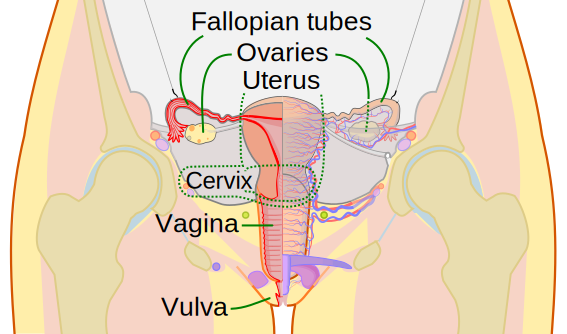
\includegraphics[width=0.7\linewidth]{./figures/reproductive_system/Scheme_female_reproductive_system-en} 

}

\caption{\href{https://commons.wikimedia.org/wiki/File:Female_anatomy_en.svg}{Diagram of the female reproductive system.}}\label{fig:femalereproductivesystem}
\end{figure}

The vagina meets the outside at the vulva, which also includes the labia, clitoris and urethra; during intercourse this area is lubricated by mucus secreted by the Bartholin's glands. The vagina is attached to the uterus through the cervix, while the uterus is attached to the ovaries via the Fallopian tubes. Each ovary contains hundreds of egg cells or ova (singular ovum).



\begin{figure}

{\centering \includegraphics[width=0.7\linewidth]{./figures/reproductive_system/Figure_28_02_02} 

}

\caption{\href{https://commons.wikimedia.org/wiki/File:Figure_28_02_02.jpg}{External and internal views of the vulva.}}\label{fig:vulvaview}
\end{figure}

Approximately every 28 days, the pituitary gland releases a hormone that stimulates some of the ova to develop and grow. One ovum is released and it passes through the Fallopian tube into the uterus. Hormones produced by the ovaries prepare the uterus to receive the ovum. The lining of the uterus, called the endometrium, and unfertilized ova are shed each cycle through the process of menstruation. If the ovum is fertilized by sperm, it attaches to the endometrium and the fetus develops.



\begin{figure}

{\centering \includegraphics[width=0.7\linewidth]{./figures/reproductive_system/Figure_28_02_07} 

}

\caption{\href{https://upload.wikimedia.org/wikipedia/commons/f/f3/Figure_28_02_07.jpg}{The progression of the menstrual cycle and the different hormones regulating it.}}\label{fig:menstrualcycle}
\end{figure}

\hypertarget{the-male-reproductive-system}{%
\section{The Male Reproductive System}\label{the-male-reproductive-system}}

The male reproductive system is a series of organs located outside the body and around the pelvis region of a male that contribute towards the reproduction process. The primary direct function of the male reproductive system is to provide the male sperm for fertilization of the ovum.



\begin{figure}

{\centering \includegraphics[width=0.7\linewidth]{./figures/reproductive_system/male anatomy} 

}

\caption{\href{https://commons.wikimedia.org/wiki/File:Male_anatomy_en.svg}{Diagram of the male reproductive system.}}\label{fig:malereproductivesystem}
\end{figure}

The major reproductive organs of the male can be grouped into three categories. The first category produces and stores sperm (spermatozoa). These are produced in the testes, which are housed in the temperature-regulating scrotum; immature sperm then travel to the epididymis for development and storage. The second category are the ejaculatory fluid producing glands which include the Cowper's gland (also called bulbo-urethral gland), seminal vesicles, prostate, and vas deferens. The final category are those used for copulation and deposition of the sperm within the female; these include the penis, urethra, and vas deferens.



\begin{figure}

{\centering \includegraphics[width=0.7\linewidth]{./figures/reproductive_system/Figure_28_01_03} 

}

\caption{\href{https://commons.wikimedia.org/wiki/File:Figure_28_01_03.JPG}{Diagram of inner structures of testes.}}\label{fig:testesdiagram}
\end{figure}

Major secondary sexual characteristics include: larger, more muscular stature, deepened voice, facial and body hair, broad shoulders, and development of an Adam's apple. An important sexual hormone of males is androgen, and particularly testosterone.

The testes release a hormone that controls the development of sperm. This hormone is also responsible for the development of physical characteristics in men such as facial hair and a deep voice.

The development of the reproductive system and the development of the urinary system are closely tied in with the development of the human fetus. Despite the differences between the adult female and male are derived from the intermediate mesoderm. The three main fetal precursors of the reproductive organs are the Wolffian duct, the Müllerian ducts, and the gonads. Endocrine hormones are a well-known and critical controlling factor in the normal differentiation of the reproductive system.



\begin{figure}

{\centering \includegraphics[width=0.7\linewidth]{./figures/reproductive_system/2915_Sexual_Differentation-02} 

}

\caption{\href{https://commons.wikimedia.org/wiki/File:2915_Sexual_Differentation-02.jpg}{Differentiation of the male and female reproductive systems from a common origin.}}\label{fig:differentiationrepsys}
\end{figure}

The Wolffian duct forms the epididymis, vas deferens, ductus deferens, ejaculatory duct, and seminal vesicle in the male reproductive system, but essentially disappears in the female reproductive system. The reverse is true for the Müllerian duct, as it essentially disappears in the male reproductive system and forms the Fallopian tubes, uterus, and vagina in the female system. In both sexes the gonads go on to form the testes and ovaries; because they are derived from the same undeveloped structure, they are considered homologous organs. There are a number of other homologous structures shared between male and female reproductive systems. However, despite the similarity in function of the female Fallopian tubes and the male epididymis and vas deferens, they are not homologous but rather analogous structures as they arise from different fetal structures.

Gametes are produced within the gonads through a process known as gametogenesis. This occurs when certain types of germ cells undergo meiosis to split the normal diploid number of chromosomes (n=46) into haploid cells containing only 23 chromosomes.



\begin{figure}

{\centering \includegraphics[width=0.7\linewidth]{./figures/reproductive_system/Normal_spermatogenesis,_intermed._mag} 

}

\caption{\href{https://commons.wikimedia.org/wiki/File:Normal_spermatogenesis,_intermed._mag.jpg}{Normal spermatogenesis, testis biopsy.}}\label{fig:testesbiopsy}
\end{figure}

In males, this process is known as spermatogenesis, and takes place only after puberty in the seminiferous tubules of the testes. The immature spermatozoa or sperm are then sent to the epididymis, where they gain a tail, enabling motility. Each of the original diploid germ cells or primary spermatocytes forms four functional gametes. The production and survival of sperms require a temperature below the normal core body temperature. Since the scrotum, where the testes is present, is situated outside the body cavity, it provides a temperature about 3 °C below normal body temperature.



\begin{figure}

{\centering \includegraphics[width=0.7\linewidth]{./figures/reproductive_system/Figure_28_01_04} 

}

\caption{\href{https://commons.wikimedia.org/wiki/File:Figure_28_01_04.jpg}{The process of spermatogenesis as the cells progress from primary spermatocytes, to secondary spermatocytes, to spermatids, to Sperm.}}\label{fig:spermatogenesis}
\end{figure}

In females, gametogenesis is known as oogenesis; this occurs in the ovarian follicles of the ovaries. This process does not produce mature ovum until puberty. In contrast with males, each of the original diploid germ cells or primary oocytes will form only one mature ovum, and three polar bodies which are not capable of fertilization. It has long been understood that in females, unlike males, all of the primary oocytes ever found in a female will be created prior to birth, and that the final stages of ova production will then not resume until puberty. However, recent scientific research has challenged that hypothesis. This new research indicates that in at least some species of mammal, oocytes continue to be replenished in females well after birth.



\begin{figure}

{\centering \includegraphics[width=0.7\linewidth]{./figures/reproductive_system/Ovarian_cortex_in_a_rhesus_monkey} 

}

\caption{\href{https://en.wikipedia.org/wiki/File:Ovarian_cortex_in_a_rhesus_monkey.jpg}{Micrograph of the ovarian cortex from a rhesus monkey showing several round follicles embedded in a matrix of stromal cells. A secondary follicle sectioned through the nucleus of an oocyte is at the upper left, and earlier stage follicles are at the lower right. The tissue was stained with the dyes hematoxylin and eosin.}}\label{fig:ovariancortex}
\end{figure}



\begin{figure}

{\centering 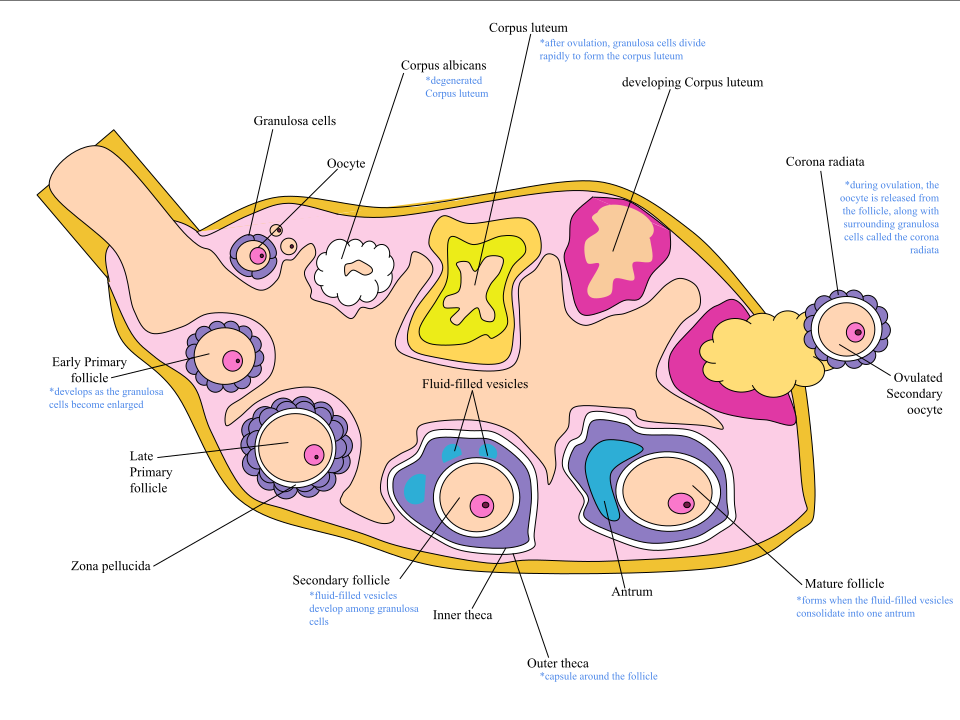
\includegraphics[width=0.7\linewidth]{./figures/reproductive_system/Oogenesis_Labeled} 

}

\caption{\href{https://commons.wikimedia.org/wiki/File:Oogenesis_Labeled.svg}{The process of ovulation and gamete production, oogenesis, in a human ovary.}}\label{fig:oogenesis}
\end{figure}


